% !TEX TS-program = xelatex%

\documentclass[aps, prd
, preprint
%, twocolumn
, nofootinbib 
, notitlepage
, superscriptaddress
, longbibliography
]{revtex4-1}
\usepackage{graphicx}
\usepackage{xcolor}
\usepackage[caption=false]{subfig}
\usepackage{mathrsfs}
\usepackage{amsmath,amssymb}
\usepackage{bm}
\usepackage{braket}
\usepackage{listings}
\usepackage{cases}
\usepackage{comment}
\usepackage{soul}
\usepackage{cancel}
\usepackage{cases}
\usepackage[utf8]{inputenc}
\usepackage{url}
\usepackage{longtable}
\usepackage[normalem]{ulem}
\usepackage[colorlinks=true
,urlcolor=blue
,anchorcolor=blue
,citecolor=blue
,filecolor=blue
,linkcolor=blue
,menucolor=blue
%,pagecolor=blue
,linktocpage=true
,pdfproducer=medialab
,pdfa=true
]{hyperref}

%\usepackage{mathpazo}
%\usepackage[no-math]{fontspec}
%\setmainfont{Palatino}
%\setsansfont{Optima}

\definecolor{MIDNIGHTBLUE}{HTML}{2C3E50}
\definecolor{ASBESTOS}{HTML}{7F8C8D}
\definecolor{TURQUOISE}{HTML}{1ABC9C}
\definecolor{PETERRIVER}{HTML}{3498DB}

\lstset{
	backgroundcolor={\color{MIDNIGHTBLUE}},
 	breaklines = true,
 	basicstyle = {\ttfamily\scriptsize\color{white}},
 	commentstyle = {\color{ASBESTOS}},
 	classoffset = 0,
 	keywordstyle = {\color{TURQUOISE}},
 	stringstyle = {\color{PETERRIVER}},
 	frame = single,
	framesep = 10pt,
 	numbers = left,
 	stepnumber = 1,
	numbersep = 15pt,
 	numberstyle = {\tiny,\color{black}},
 	tabsize = 4,
 	captionpos = t
}

\newcommand{\dif}[2]{\frac{\mathrm{d} #1}{\mathrm{d} #2}}
\newcommand{\pdif}[2]{\frac{\partial #1}{\partial #2}}
\newcommand{\var}[2]{\frac{\delta #1}{\delta #2}}
\newcommand{\dd}{\mathrm{d}}
\newcommand{\DD}{\mathscr{D}}
\newcommand{\ee}{\mathrm{e}}
\newcommand{\diag}{\mathrm{diag}}
\newcommand{\sgn}{\mathrm{sgn}}
\newcommand{\Mpl}{M_\text{Pl}}
\newcommand{\ns}{n_{{}_\mathrm{S}}}
\newcommand{\cs}{c_{{}_\mathrm{S}}}
\newcommand{\IR}{\text{IR}}
\newcommand{\UV}{\text{UV}}
\renewcommand{\Re}{\mathrm{Re}}
\renewcommand{\Im}{\mathrm{Im}}
\newcommand{\dk}{\frac{\dd^3k}{(2\pi)^3}}
\newcommand{\bbalpha}{{\alpha\!\!\!\alpha}}
\newcommand{\dps}{\displaystyle}
\newcommand{\SIA}{S_\text{IA}}
\newcommand{\eff}{\text{eff}}
\newcommand{\kdx}{\mathbf{k}\cdot\mathbf{x}}

\newcommand{\calC}{\mathcal{C}}
\newcommand{\calD}{\mathcal{D}}
\newcommand{\scrD}{\mathscr{D}}
\newcommand{\calg}{\mathcal{g}}
\newcommand{\calH}{\mathcal{H}}
\newcommand{\scrH}{\mathscr{H}}
\newcommand{\uI}{\text{I}}
\newcommand{\calJ}{\mathcal{J}}
\newcommand{\scrJ}{\mathscr{J}}
\newcommand{\calL}{\mathcal{L}}
\newcommand{\scrL}{\mathscr{L}}
\newcommand{\calM}{\mathcal{M}}
\newcommand{\calN}{\mathcal{N}}
\newcommand{\calO}{\mathcal{O}}
\newcommand{\scrO}{\mathscr{O}}
\newcommand{\calP}{\mathcal{P}}
\newcommand{\calR}{\mathcal{R}}
\newcommand{\uR}{\text{R}}

\newcommand{\bae}[1]{\begin{align} #1 \end{align}}
\newcommand{\bce}[1]{\begin{cases} #1 \end{cases}}
\newcommand{\bfe}[4]{
\begin{figure} 
	\centering
	\includegraphics[#1]{#2}
	\caption{#3}
	\label{#4}
\end{figure}}
\newcommand{\bpme}[1]{\begin{pmatrix} #1 \end{pmatrix}}

\newcommand{\Red}[1]{\textcolor{red}{\sffamily #1}}
\newcommand{\Mag}[1]{\textcolor{magenta}{\sffamily #1}}
\newcommand{\Blue}[1]{\textcolor{blue}{\sffamily #1}}
\newcommand{\mathblue}[1]{\textcolor{blue}{#1}}
\newcommand{\YT}[1]{\textcolor{blue}{\sffamily [YT : #1]}}



\begin{document}
\title{User's guide for \textsc{StocDeltaN}}% \\[-10pt] {- \small\textit{field-space type} -}}
\date{\today}

%\author{S\'ebastien Renaux-Petel}
%\email{renaux@iap.fr}
%\affiliation{Institut d'Astrophysique de Paris, UMR 7095 du CNRS et Sorbonne Universit\'e, 
%98bis boulevard Arago, 75014 Paris, France}
\author{Yuichiro Tada}
\email{tada.yuichiro@e.mbox.nagoya-u.ac.jp}
\affiliation{Department of Physics, Nagoya University, Nagoya 464-8602, Japan}
%\author{Vincent Vennin}
%\email{vincent.vennin@apc.univ-paris7.fr}
%\affiliation{Laboratoire Astroparticule et Cosmologie, Universit\'e Denis Diderot Paris 7, 
%10 rue Alice Domon et L'eonie Duquet, 75013 Paris, France}


%\begin{abstract}
%\end{abstract}

\maketitle
%\tableofcontents

%\vspace{-30pt}
\section{Code Overview}

\textsc{StocDeltaN} is a powerful C++ package to analyze inflationary dynamics and calculate the power spectrum of curvature perturbations with use of the techniques of 
the stochastic-$\delta N$ approach~\cite{Fujita:2013cna,Vennin:2015hra}. 
This automatically includes resummation effects of superhorizon perturbations, enabling a non-perturbative approach to the curvature perturbation.
This package is applicable to general multi-field models in non-trivial field spaces expressed by the general Lagrangian~(\ref{eq: Lagrangian}).
\textsc{StocDeltaN} supports the full phase-space analysis by solving both the inflaton fields $\phi^I$ and their conjugate momenta $\pi_I$, while it automatically switch to the slow-roll field-space analysis if users do not specify the calculation box for the momenta.
Though the slow-roll approximation may fail in some cases, it is computationally much more economic and often enough for leading order calculations.

\begin{comment}
We provide two types of StocDeltaN: one is the full phase-space formulation time without the slow-roll approximation,
while the other is the field-space formulation omitting the degrees of freedom (d.o.f.) of inflaton momenta under the slow-roll approximation.
Though the latter, which is labeled by ``\_conf" \Blue{(meaning of ``configuration". to be renamed?)}, sometimes wrong in models where e.g. the slow-roll conditions are violated for an instant,
it is much more economic computationally thanks to the halved d.o.f. and often enough for leading order calculations.
In this user's guide, we focus on this field-space type though the usage is naturally extended to the phase-space type.
\end{comment}

\textsc{StocDeltaN} consists of two parts as the \emph{source} part containing all required numerical solvers which we provide and the \emph{main} part where users specify the inflationary model
and the usage of several options like a plotting option with use of Python. Users can write the \emph{main} code using various sample codes as references.

The \emph{source} part in itself is divided into three parts as \texttt{JacobiPDE}, \texttt{SRK32}, and \texttt{StocDeltaN}.
\texttt{JacobiPDE} and \texttt{SRK32} implement the solver classes for partial differential equations (PDE) and stochastic differential equations (SDE) respectively.
Overriding these classes, users can employ the numerical solver for general problems beyond the inflationary system if want.
\texttt{StocDeltaN} overrides their classes and defines the specific class as the stochastic-$\delta N$ solver.
The \emph{main} code specifies the inflationary model, overriding its functions defining e.g. potential, field-space metric, and so on,
and then user can use its member functions to analyze the stochastic inflation.

\newpage


\section{Tutorials}

\subsection{Prerequisties}

\begin{itemize}
\item {\sffamily\bfseries C++ compiler} : We have checked the operation in GNU, Clang, and Intel compiler on Mac system. GNU compiler will be used by default.
On Mac system, generally Clang compiler is preinstalled and automatically called instead of GNU compiler, so users need not to install other compilers by themselves. 
By modifying Makefile, one can change the used compiler if wants.

\item {\sffamily\bfseries Make} : For an easy compilation, \textsc{StocDeltaN} employs Make which is a compilation manager. On Mac system, it is easy to introduce GNU Make
by installing Command Line Tools of Xcode.

\item {\sffamily\bfseries OpenMP (optional)} : The modern concept of processor design places importance on parallelization over multicore rather than processing power on each single core. 
Multicore processors are implemented even on personal computers and parallelization gets much closer to end users.
\textsc{StocDeltaN} employs automatic parallelization with use of OpenMP. Many representative compilers like GNU or Intel's one precontain OpenMP, and therefore
users can make use of its parallelization simply by validating OpenMP option (e.g. -fopenmp for GNU compiler) in Makefile.
Clang compiler preinstalled on Mac may not support OpenMP, then OpenMP option is commented out in a sample Makefile.
But we strongly recommend the usage of OpenMP to bring out the full performance of \textsc{StocDeltaN} particularly in calculation on cluster computers.

\item{\sffamily\bfseries Python \& Matplotlib (optional)} : Though \textsc{StocDeltaN} exports all relevant data as DAT files, one can also use the automatic plotting system
with use of Matplotlib which is Python's plotting library. Piping data to python, \textsc{StocDeltaN} can plot the obtained results if Python and Matplotlib have been installed
on a user's machine. Mac system has usually preinstalled Python, and therefore one can easily install Matplotlib as well by using Pip Installs Packages, e.g.
\begin{lstlisting}[language = bash, numbers = none]
$ pip install matplotlib
\end{lstlisting}

\end{itemize}


\subsection{First Exercise}

Practice makes perfect. 
Let us start by downloading the source codes from our GitHub page \url{https://github.com/NekomammaT/StocDeltaN_dist} and play with attached samples.
Using Make in the \textit{sample} directory completes the compilation of the sample codes:
\begin{lstlisting}[language = bash, numbers = none]
$ cd sample
$ make
\end{lstlisting}
By default the field-space double chaotic model (\emph{double\_chaotic\_SR.cpp}) is compiled. Then running the executable file, one obtains some results like as follows.
\begin{lstlisting}[language = bash, numbers = none]
$ ./double_chaotic_SR
[xi, xf, xmin, xmax]:
[13, 3.54334e-08, -5.06876e-07, 13]
[13, 1.40077, 1.40077, 13]

N = 84.01
Vi = 8.5543209876543225e-09,  Vf = 1.2111996327249413e-12
0.190044 sec.
\end{lstlisting}
If you could do this without any error, the machine environment is properly set up and you are ready to execute a main calculation.

One edits the following parts of \textit{double\_chaotic\_SR.cpp}. Simply by commenting out \texttt{sdn.sample()} and validating \texttt{sdn.solve()} instead as 
indicated in List.~\ref{list: double_chaotic_SR_plot} \YT{modify comments},
one can fully solve the system.
Re-Making and running \textit{double\_chaotic\_SR}, one obtains the analyzation results in 
\textit{Mn\_double\_chaotic\_SR.dat}, \textit{traj\_double\_chaotic\_SR.dat},
and \textit{calP\_double\_chaotic\_SR.dat}, which contain the data as shown in Lists.~\ref{list: Mn_double_chaotic_SR.dat}--\ref{list: calP_double_chaotic_SR.dat}.

\begin{lstlisting}[language = C++, caption=\textit{sample/double\_chaotic\_SR.cpp}, label = list: double_chaotic_SR_plot, firstnumber = 77]
	//sdn.sample(); // obtain 1 sample path
	//sdn.sample_plot(); // plot that sample path 
	
	sdn.solve(); // solve PDE & SDE and obtain power spectrum  
	//sdn.f_plot(0); // show plot of <N>
	//sdn.f_plot(1); // show plot of <delta N^2> 
	//sdn.calP_plot(); // show plot of power spectrum of zeta
\end{lstlisting}

\vfill

\begin{lstlisting}[numbers = none, mathescape, caption={\textit{Mn\_}$\braket{\text{model name}}$\textit{.dat} : 
contour data of $\calM_n=\braket{\calN^n}$ and $\calC_2=\braket{\delta\calN^2}$}, label = list: Mn_double_chaotic_SR.dat]
$\phi^1$ $\phi^2$ $\cdots$ $\pi_1$ $\pi_2$ $\cdots$ $\calM_1$ $\calC_2$
\end{lstlisting}

\begin{lstlisting}[numbers = none, mathescape, caption={\textit{traj\_}$\braket{\text{model name}}$\textit{.dat} : trajectory data of one sample path}, 
label = list: traj_double_chaotic_SR.dat]
$N$ $\phi^1$ $\phi^2$ $\cdots$ $\pi_1$ $\pi_2$ $\cdots$
\end{lstlisting}

\begin{lstlisting}[numbers = none, mathescape, caption={\textit{calP\_}$\braket{\text{model name}}$\textit{.dat} : data related to curvature perturbation}, 
label = list: calP_double_chaotic_SR.dat]
$\braket{\calN}$ $\braket{\delta\calN^2}$ $\calP_\zeta$
\end{lstlisting}

If you have installed Python and Matplotlib already, the plotting option is quite useful.
Validating \texttt{sdn.f\_plot(0)}, \texttt{sdn.f\_plot(1)}, and \texttt{sdn.calP\_plot()} shown in List.~\ref{list: double_chaotic_SR_plot},
\textsc{StocDeltaN} pipes the data to Python and plots contours of $\calM_1=\braket{\calN}$ and $\calC_2=\braket{\delta\calN^2}$ 
and the power spectrum of curvature perturbations $\calP_\zeta$ as shown in
Fig.~\ref{fig: double_chaotic_conf}. The plots are also saved as \textit{N\_double\_chaotic\_SR.pdf}, \textit{dN2\_double\_chaotic\_SR.pdf}, and
\textit{calP\_double\_chaotic\_SR.pdf}.
See Sec.~\ref{sec: StocDeltaN} for more details about the plotting functions.

\begin{figure}
	\centering
	\begin{tabular}{ccc}
		\begin{minipage}{0.33\hsize}
			\centering
			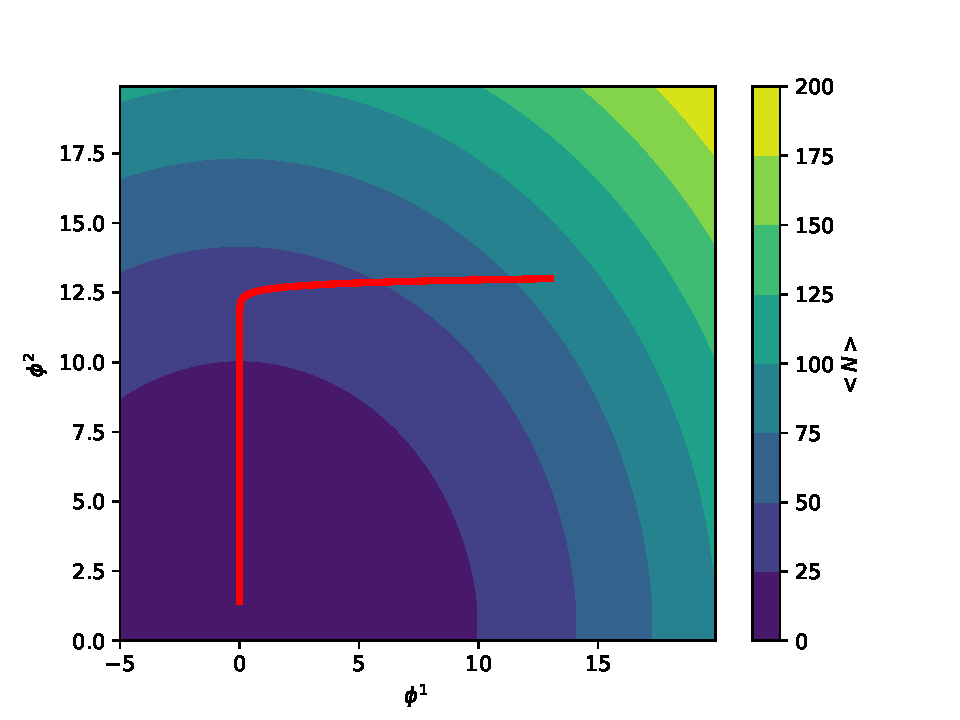
\includegraphics[width=\hsize]{figs/N_double_chaotic_conf.pdf}
		\end{minipage}
		\begin{minipage}{0.33\hsize}
			\centering
			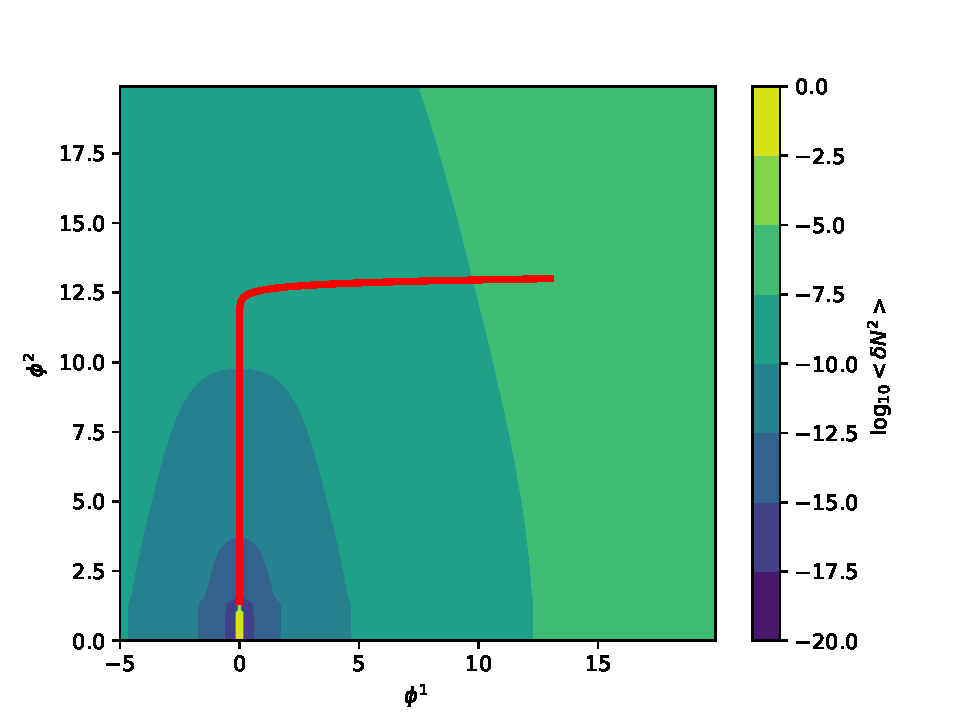
\includegraphics[width=\hsize]{figs/dN2_double_chaotic_conf.pdf}
		\end{minipage}
		\begin{minipage}{0.33\hsize}
			\centering
			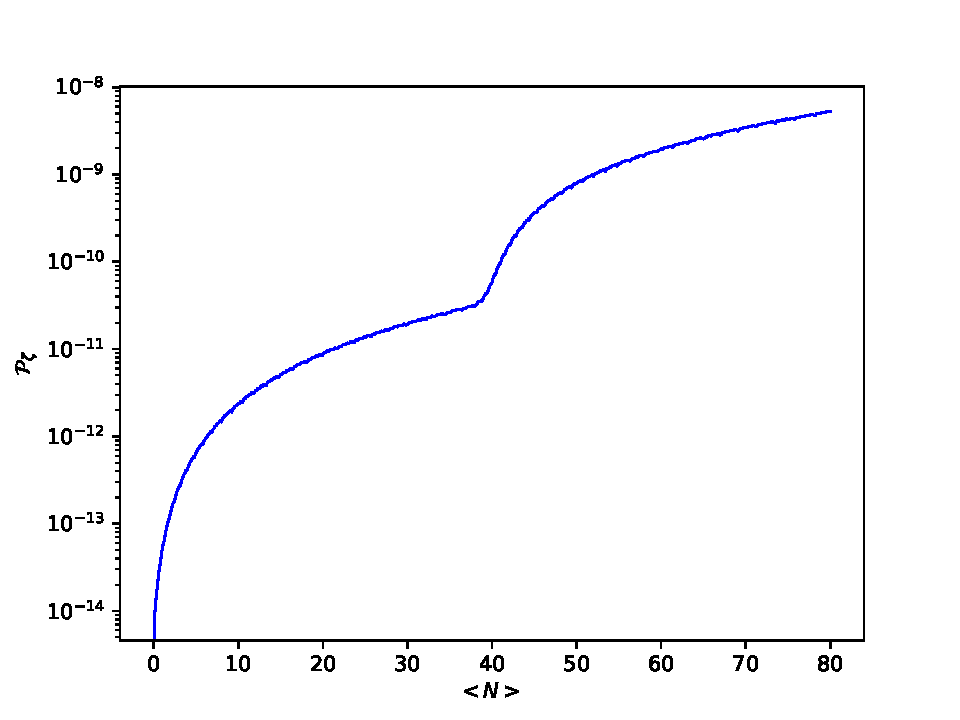
\includegraphics[width=\hsize]{figs/calP_double_chaotic_conf.pdf}
		\end{minipage}
	\end{tabular}
	\caption{\textit{N\_double\_chaotic\_SR.pdf}, \textit{dN2\_double\_chaotic\_SR.pdf}, and \textit{calP\_double\_chaotic\_SR.pdf} from left to right.
	Red lines in the left and middle panels show one realization of sample paths.}
	\label{fig: double_chaotic_conf}
\end{figure}

To switch the analyzed model, one modifies \textit{Makefile} in the \textit{sample} directory. The \texttt{MODEL} parameter in \textit{Makefile} 
as can be seen in List.~\ref{list: Makefile} controls the analyzed model and one can calculate other models by changing this parameter.
We preprovided five other models, \textit{chaotic\_SR} \textit{chaotic}, \textit{hilltop\_SR}, \textit{hilltop}, and \textit{hybrid\_SR}, as samples.
One can use preferred C++ compiler by changing \texttt{CXX} parameter. The default setting is GNU compiler \texttt{g++} (On Mac system, it basically calls 
Clang compiler instead which may not support OpenMP. That is why we comment out OpenMP option \texttt{-fopenmp} by default).
If you use a compiler supporting OpenMP, you may use it by validating the OpenMP option \texttt{-fopenmp} (or \texttt{-qopenmp} for Intel compiler).

\begin{lstlisting}[language = bash, caption={\textit{sample/Makefile}}, label=list: Makefile]
MODEL = double_chaotic_SR
SOURCE = ../source

CXX := g++
CXXFLAGS := -std=c++11 -O3 #-fopenmp
\end{lstlisting}



\subsection{Beyond samples}

Of course the final goal is not playing with sample codes but solving your models. Though ultimately the understanding of the whole code structure is required
to get a full command of \textsc{StocDeltaN}, we recommend to take advantage of sample codes as much as possible. That is, if you want to solve single-field models in the slow-roll (SR) limit,
\textit{chaotic\_SR.cpp} or \textit{hilltop\_SR.cpp} would be helpful, while \textit{double\_chaotic\_SR.cpp} or \textit{hybrid\_SR.cpp} can be used for two-field models. \textit{chaotic.cpp} or \textit{hilltop.cpp} would be a reference for the phase-space approach.
To adopt your model to \textsc{StocDeltaN}, you change the code in mainly two senses: one is the inflaton's system described by the Lagrangian, and the other is 
the numerical parameters used for practical calculations. We guide the readers in this way below.


\subsubsection{Lagrangian}

\textsc{StocDeltaN} supports general multi-scalar models in general relativity. Such models are parameterized the following scalar part Lagrangian.
\bae{\label{eq: Lagrangian}
	\calL=-\frac{1}{2}G_{IJ}(\phi)\partial_\mu\phi^I\partial^\mu\phi^J-V(\phi).
}
Here $I$ and $J$ label the scalar fields and $G_{IJ}$ represents the inflaton's field space metric which can be curved in general.
The conjugate momenta for the phase-space approach are defined by \YT{$G_{IJ}\dif{\phi^J}{N}$ is better?}
\bae{
    \pi_I=G_{IJ}\dot{\phi}^J. 
}

This Langrangian is set in \textsc{StocDeltaN} by the corresponding functions in a main code represented by e.g. \textit{double\_chaotic\_SR.cpp}
as shown in List.~\ref{list: double_chaotic_SR_lag}.
Each function represent:
\begin{itemize}
\item \texttt{V(X)} : the inflaton potential $V(\phi)$.
\item \texttt{VI(X,I)} : its derivative $\partial_{\phi^I}V(\phi)$.
\item \texttt{metric(X,I,J)} : the field space metric $G_{IJ}(\phi)$.
\item \texttt{inversemetric(X,I,J)}: its inverse $G^{IJ}(\phi)$.
\item \texttt{affine(X,I,J,K)} : the Christoffel symbol corresponding to the field space metric, $\Gamma^I_{JK}(\phi)=\frac{1}{2}G^{IL}(G_{JL,K}+G_{KL,J}-G_{JK,L})$.
\item \texttt{derGamma(X,I,J,K,L)} : its derivative $\partial_{\phi^L}\Gamma^I_{JK}$.
\end{itemize}
\textit{double\_chaotic\_SR.cpp} studies the double mass-term inflation with a flat field space as
\bae{
	V=\frac{1}{2}M^2\phi^2+\frac{1}{2}m^2\psi^2, \qquad G_{IJ}=\delta_{IJ}.
}
In the code the list \texttt{X} represents the scalar fields as $\texttt{X[0]}=\phi$ and $\texttt{X[1]}=\psi$, then the functions are defined as shown 
in List.~\ref{list: double_chaotic_SR_lag} \YT{modify the line number and comments}. The potential parameters $M$ and $m$ are defined at the top of the code as \texttt{MPHI} and \texttt{MPSI} to be easily modified.
Therefore one can adopt the model interested simply by rewriting this part.

\begin{lstlisting}[language = C++, caption={\textit{sample/double\_chaotic\_SR.cpp}}, label=list: double_chaotic_SR_lag, firstnumber = 20]
// ---------- potential parameter ----------
#define MPHI (1e-5)
#define MPSI (MPHI/9.)
// -----------------------------------------
\end{lstlisting}

\begin{lstlisting}[language = C++, firstnumber = 93]
// ---------- Lagrangian params. and diff. coeff.  X[0]=phi, X[1]=psi ----------

double StocDeltaN::V(vector<double> &X)
{
  return 1./2*MPHI*MPHI*X[0]*X[0] + 1./2*MPSI*MPSI*X[1]*X[1];
}

double StocDeltaN::VI(vector<double> &X, int I) // \partial_I V
{
  if (I == 0) {
    return MPHI*MPHI*X[0];
  } else {
    return MPSI*MPSI*X[1];
  }
}

double StocDeltaN::metric(vector<double> &X, int I, int J) // G_IJ
{
  if (I == J) {
    return 1;
  } else {
    return 0;
  }
}

double StocDeltaN::inversemetric(vector<double> &X, int I, int J) // G^IJ
{
  return metric(X,I,J);
}

double StocDeltaN::affine(vector<double> &X, int I, int J, int K) // \Gamma^I_JK
{
  return 0;
}

double StocDeltaN::derGamma(vector<double> &X, int I, int J, int K, int L)
{
  return 0;
}
\end{lstlisting}


\subsubsection{lattice size}

The other important parameter for \textsc{StocDeltaN} is the lattice size defining the inflationary region.
\textsc{StocDeltaN} adopts the orthogonal box with arbitrary variable lattice steps as shown in Fig.~\ref{fig: box}.
The box can include the non-inflationary region where the corresponding energy density is lower than the threshold $\rho_c$
shown by the blue shade in Fig.~\ref{fig: box}, other than the yellow inflationary region $\Omega$.
Note that the boundaries of $\Omega$ other than the end of inflation $\rho_c$ are unphysical. \textsc{StocDeltaN} sets the reflecting boundary condition for them by default but users should choose the boundary position so that the relevant region is sufficiently far from those unphysical boundaries.

The box is parametrized by 3-dimensional list containing the field values of lattice sites in each scalar direction, i.e.,
\begin{lstlisting}[numbers = none, mathescape]
{{{$\phi_0$, $\phi_1$, $\phi_2$, $\cdots$, $\phi_\text{max}$}, {$\psi_0$, $\psi_1$, $\psi_2$, $\cdots$, $\psi_\text{max}$}}}
\end{lstlisting}
for the SR field-space approach, while the lattice sites for the momenta as
\begin{lstlisting}[numbers = none, mathescape]
{{{$\phi_0$, $\phi_1$, $\phi_2$, $\cdots$, $\phi_\text{max}$}, {$\psi_0$, $\psi_1$, $\psi_2$, $\cdots$, $\psi_\text{max}$}},
 {{$\pi_{\phi0}$, $\pi_{\phi1}$, $\pi_{\phi2}$, $\cdots$, $\pi_{\phi\text{max}}$}, {$\pi_{\psi0}$, $\pi_{\psi1}$, $\pi_{\psi2}$, $\cdots$, $\pi_{\psi\text{max}}$}}}
\end{lstlisting}
for the full phase-space approach
in the case of Fig.~\ref{fig: box}.
\textsc{StocDeltaN} automatically switches the approach, according to the presence of the lattice for momenta.

\bfe{width=0.9\hsize}{figs/box.pdf}{Schematic image of the calculable lattice in \textsc{StocDeltaN}. Users declare each field value 
$\phi_0$, $\phi_1$, $\phi_2$, $\cdots$, $\phi_\text{max}$, and $\psi_0$, $\psi_1$, $\psi_2$, $\cdots$, $\psi_\text{max}$.}{fig: box}

In \textit{double\_chaotic\_SR.cpp}, the box boundary is defined by \texttt{PHIMIN}, \texttt{PHIMAX}, \texttt{PSIMIN}, and \texttt{PSIMAX}
with the constant lattice steps \texttt{HPHI} and \texttt{HPSI}, declared at the top of the code as shown in List.~\ref{list: double_chaotic_conf_box}.
The concrete 3-dimensional list is created in the latter part as \texttt{sitepack}.

\begin{lstlisting}[language = C++, caption={\textit{sample/double\_chaotic\_SR.cpp}}, label=list: double_chaotic_conf_box, firstnumber = 6]
// ---------- box size & step h ------------
#define PHIMIN -5
#define PHIMAX 20
#define PSIMIN 0
#define PSIMAX 20
#define HPHI (1e-1)
#define HPSI (1e-1)
// -----------------------------------------
\end{lstlisting}
\begin{lstlisting}[language = C++, firstnumber = 52]
	// ---------- set box step h ---------------
	double h = HPHI, sitev = PHIMIN;
	vector<double> site;
	vector< vector<double> > xsite;
	vector< vector< vector<double> > > sitepack;
	while (sitev <= PHIMAX) {
		site.push_back(sitev);
		sitev += h;
	}
	xsite.push_back(site);
	site.clear();

	h = HPSI, sitev = PSIMIN;
	while (sitev <= PSIMAX) {
		site.push_back(sitev);
		sitev += h;
	}
	xsite.push_back(site);
	site.clear();
	
	sitepack.push_back(xsite);
	xsite.clear();
	// -----------------------------------------
\end{lstlisting}

One might prefer the logarithmic lattice to the constant step size. In such a case, it is useful to determine the step size by the field value itself.
\textit{hybrid\_SR.cpp} employs this procedure in $\psi$'s direction.
In line \Blue{70} shown in List.~\ref{list: hybrid_conf_box}, the step size in $\psi$'s direction is determined by its $\psi$-value itself with a fraction \texttt{HPSIOPSI}
and the lower bound \texttt{HPSIMIN}. Therefore the lattice step size becomes smaller for the smaller value of $|\psi|$, resulting in the logarithmic scale.

\begin{lstlisting}[language = C++, caption={\textit{sample/hybrid\_SR.cpp}}, label=list: hybrid_conf_box, firstnumber = 6]
// ---------- box size & step h ------------
#define PHIMIN 0.1409
#define PHIMAX 0.142
#define PSIMIN -(1e-3)
#define PSIMAX (1e-3)
#define HPHI (1e-5)
#define HPSIOPSI (1e-2) // hpsi/|psi|
#define HPSIMIN (1e-10)
// -----------------------------------------
\end{lstlisting}
\begin{lstlisting}[language = C++, firstnumber = 57]
	// ---------- set box step h ---------------
	double h = HPHI, sitev = PHIMIN;
	vector<double> site;
	vector< vector<double> > xsite;
	vector< vector< vector<double> > > sitepack;
	while (sitev <= PHIMAX) {
		site.push_back(sitev);
		sitev += h;
	}
	xsite.push_back(site);
	site.clear();

	sitev = PSIMIN;
	while (sitev <= PSIMAX) {
		h = max(fabs(sitev)*HPSIOPSI,HPSIMIN);

		site.push_back(sitev);
		sitev += h;	
	}
	xsite.push_back(site);
	site.clear();
	
	sitepack.push_back(xsite);
	xsite.clear();
	// ------------------------------------------
\end{lstlisting}

\textit{chaotic.cpp} shown in List.~\ref{list: chaotic_box} will be helpful for the box declaration in the phase-space approach. The logarithmic scale is adopted for the momentum.
In any case, \texttt{site} corresponds with the most inner list, \texttt{xsite}/\texttt{xpsite} assembles the fields box or the momenta box, and \texttt{sitepack} is the full box list in our codes, but any other implementation also works as long as the final list is consistently configured as indicated in the beginning of this subsection.

\begin{lstlisting}[language = C++, caption={\textit{sample/chaotic.cpp}}, label=list: chaotic_box, firstnumber = 6]
// ---------- box size & step h ------------
#define XMIN 0
#define XMAX 15
#define PMIN (-1e-4)
#define PMAX 0
#define HX 0.01
#define HPMIN (1e-6)
#define HPOV (1./20)
// -----------------------------------------
\end{lstlisting}
\begin{lstlisting}[language = C++, firstnumber = 57]
    // ---------- set box step h ---------------
    double h = HX, sitev = XMIN;
    vector<double> site;
    vector< vector<double> > xpsite;
    vector< vector< vector<double> > > sitepack;
    while(sitev <= XMAX) {
        site.push_back(sitev);
        sitev += h;
    }
    xpsite.push_back(site);
    sitepack.push_back(xpsite);
    site.clear();
    xpsite.clear();

    sitev = PMIN;
    while (sitev <= PMAX) {
        h = max(fabs(sitev)*HPOV,HPMIN);

        site.push_back(sitev);
        sitev += h;
    }
    xpsite.push_back(site);
    sitepack.push_back(xpsite);
    site.clear();
    xpsite.clear();
    // ------------------------------------------
\end{lstlisting}


\subsubsection{other parameters}

Other parameters are set at the top of the code and gathered into the parameter list \texttt{params} which is called for the declaration of the \texttt{StocDeltaN} class. The initial condition for the inflationary trajectories is declared by \texttt{xpi} in the form of
\begin{lstlisting}[numbers = none, mathescape]
{{$\phi_i$, $\psi_i$}}    
\end{lstlisting}
or
\begin{lstlisting}[numbers = none, mathescape]
{{$\phi_i$, $\psi_i$}, {$\pi_{\phi i}$, $\pi_{\psi i}$}}
\end{lstlisting}
List.~\ref{list: double_chaotic_SR_otherparams} shows the sample code. The parameter list \texttt{params} consists of the maximal step number and tolerance for the PDE solver, the order of e-folds moment to be calculated, the energy surface of the end of inflation, the number of the independent noise degrees of freedom, e-folds time step for the trajectory calculation, the maximum and step of e-folds for the power spectrum calculation, and the recursion number of sample trajectories in the stochastic-$\delta N$ approach. The detailed explanation of these parameters can be found in the next section.

\begin{lstlisting}[language = C++, caption={\textit{sample/double\_chaotic\_SR.cpp}}, label=list: double_chaotic_SR_otherparams, firstnumber = 4]
#define MODEL "double_chaotic_SR" // model name
\end{lstlisting}
\begin{lstlisting}[language = C++, firstnumber = 15]
// ---------- for PDE ----------------------
#define MAXSTEP 100000 // max recursion
#define TOL 1e-10 // tolerance
// -----------------------------------------
\end{lstlisting}
\begin{lstlisting}[language = C++, firstnumber = 25]
#define RHOC (MPSI*MPSI) // end of inflation

// ---------- for SDE ----------------------
#define RECURSION 100 // recursion for power spectrum
#define PHIIN 13 // i.c. for phi
#define PSIIN 13 // i.c. for psi
#define TIMESTEP (1e-2) // time step: delta N
// -----------------------------------------

// ---------- for power spectrum -----------
#define DELTAN 0.1 // calc. PS every DELTAN e-folds
#define NMAX 80 // calc. PS for 0--NMAX e-folds
// -----------------------------------------
\end{lstlisting}
\begin{lstlisting}[language = C++, firstnumber = 72]
    vector<double> params = {MAXSTEP,TOL,2,RHOC,(double)sitepack[0].size(),TIMESTEP,NMAX,DELTAN,RECURSION};

    vector< vector<double> > xpi = {{PHIIN,PSIIN}}; // set i.c. for inflationary trajectories

    StocDeltaN sdn(MODEL,sitepack,xpi,0,params); // declare the system
\end{lstlisting}



\section{Code Structures}

Though the previous Tutorial section is basically enough for light users, one might desire to customize the codes for his/her own problem.
In this section, the detailed structures of three parts (\texttt{JacobiPDE}, \texttt{SRK32}, and \texttt{StocDeltaN}) are described, suggesting possible arranges.


\subsection{\texttt{JacobiPDE}}

\texttt{JacobiPDE} is the partial differential equation (PDE) solver with use of the Jacobi method.

description of Jacobi method

member function



\subsection{\texttt{SRK32}}

description of SRK32

member function


\subsection{\texttt{StocDeltaN}}\label{sec: StocDeltaN}

description of stochastic-$\delta N$

member function



%\acknowledgments





%\appendix







\bibliography{main}
\end{document}